%%%%%%%%%%%%%%%%%%%%%%%%%%%%%%%%%%%%%%%%%%%%%%%%%%%%%
% 緒言
%%%%%%%%%%%%%%%%%%%%%%%%%%%%%%%%%%%%%%%%%%%%%%%%%%%%%

\chapter{緒言}
\label{Chapter1}

緒言を書こう~\cite{bibtest}.

図の参照テスト Fig.~\ref{fig:test}.%reffig使うと太字になります

複数の画像を一つのfigure環境に入れたい場合は,subcaption環境を使いましょうFig.~\ref{fig:animals}.
こんな感じで参照も可能Fig.~\ref{fig:frog}.

\begin{figure}[tb]
  \begin{minipage}[b]{.5\columnwidth}
   \centering
   
\includegraphics[width=\columnwidth]{./figure/cat.png}
   \subcaption{Tiger}
   \label{fig:frog}
 \end{minipage}%
 \begin{minipage}[b]{.5\columnwidth}
  \centering
  
\includegraphics[width=\columnwidth]{./figure/elephant.png}
  \subcaption{Bear}
  \label{fig:gorilla}
 \end{minipage}
 \caption{犬と羊}\label{fig:animals}
\end{figure}

\begin{figure}[tb]
    \centering 
     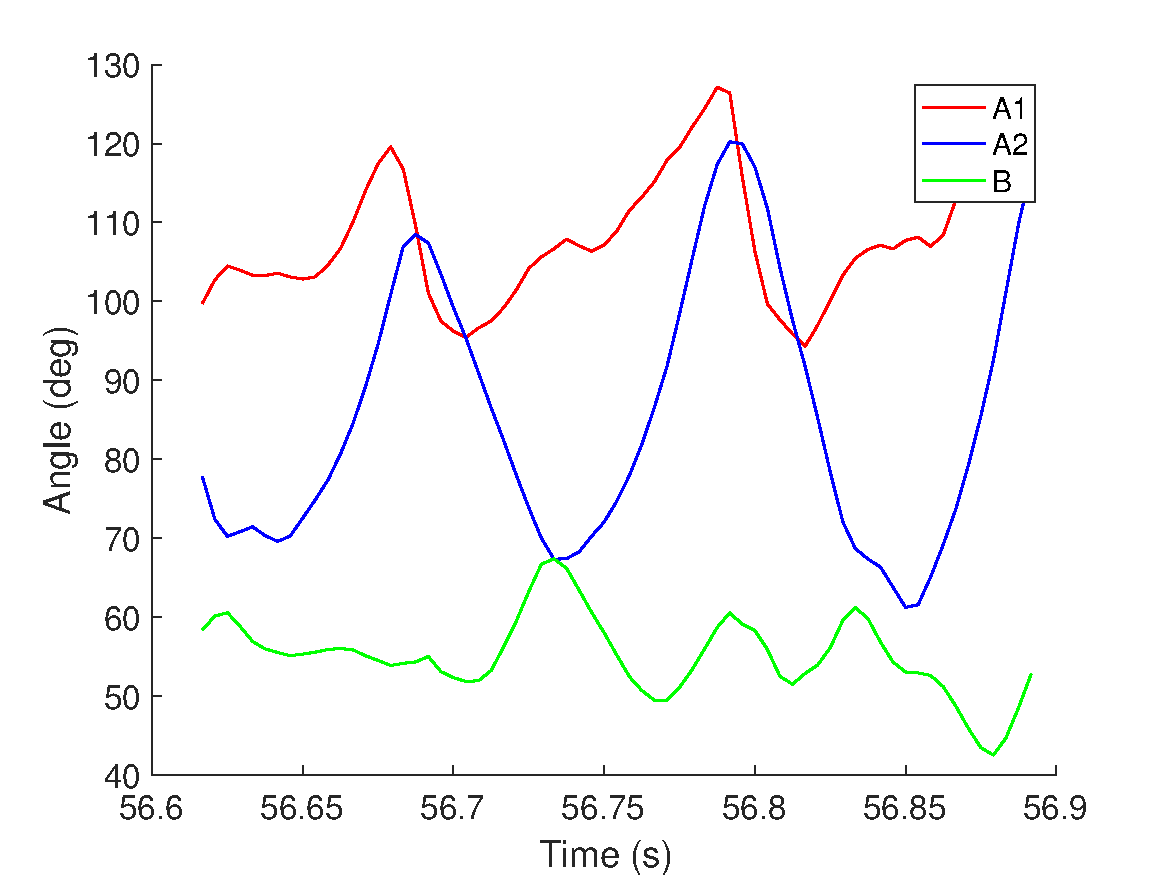
\includegraphics[width=\columnwidth]{./figure/testfig.pdf}
     \caption{キャプションを書こう}
     \label{fig:test}
\end{figure}

\begin{align}
    y=\sin{A}
    \label{eq:test}
\end{align}


ぞうの鼻はながいぞうぞうの鼻はながいぞうぞうの鼻はながいぞうぞうの鼻はながいぞうぞうの鼻はながいぞうぞうの鼻はながいぞうぞうの鼻はながいぞうぞうの鼻はながいぞうぞうの鼻はながいぞうぞうの鼻はながいぞうぞうの鼻はながいぞうぞうの鼻はながいぞうぞうの鼻はながいぞうぞうの鼻はながいぞうぞうの鼻はながいぞうぞうの鼻はながいぞうぞうの鼻はながいぞうぞうの鼻はながいぞうぞうの鼻はながいぞうぞうの鼻はながいぞうぞうの鼻はながいぞうぞうの鼻はながいぞうぞうの鼻はながいぞうぞうの鼻はながいぞうぞうの鼻はながいぞうぞうの鼻はながいぞうぞうの鼻はながいぞうぞうの鼻はながいぞうぞうの鼻はながいぞうぞうの鼻はながいぞうぞうの鼻はながいぞうぞうの鼻はながいぞうぞうの鼻はながいぞうぞうの鼻はながいぞうぞうの鼻はながいぞうぞうの鼻はながいぞうぞうの鼻はながいぞうぞうの鼻はながいぞうぞうの鼻はながいぞうぞうの鼻はながいぞうぞうの鼻はながいぞうぞうの鼻はながいぞうぞうの鼻はながいぞうぞうの鼻はながいぞうぞうの鼻はながいぞうぞうの鼻はながいぞうぞうの鼻はながいぞうぞうの鼻はながいぞうぞうの鼻はながいぞうぞうの鼻はながいぞうぞうの鼻はながいぞうぞうの鼻はながいぞうぞうの鼻はながいぞうぞうの鼻はながいぞうぞうの鼻はながいぞうぞうの鼻はながいぞうぞうの鼻はながいぞうぞうの鼻はながいぞうぞうの鼻はながいぞうぞうの鼻はながいぞうぞうの鼻はながいぞうぞうの鼻はながいぞうぞうの鼻はながいぞうぞうの鼻はながいぞうぞうの鼻はながいぞうぞうの鼻はながいぞうぞうの鼻はながいぞうぞうの鼻はながいぞうぞうの鼻はながいぞうぞうの鼻はながいぞうぞうの鼻はながいぞうぞうの鼻はながいぞうぞうの鼻はながいぞうぞうの鼻はながいぞうぞうの鼻はながいぞうぞうの鼻はながいぞうぞうの鼻はながいぞうぞうの鼻はながいぞうぞうの鼻はながいぞうぞうの鼻はながいぞうぞうの鼻はながいぞうぞうの鼻はながいぞうぞうの鼻はながいぞうぞうの鼻はながいぞうぞうの鼻はながいぞうぞうの鼻はながいぞうぞうの鼻はながいぞうぞうの鼻はながいぞうぞうの鼻はながいぞうぞうの鼻はながいぞうぞうの鼻はながいぞうぞうの鼻はながいぞうぞうの鼻はながいぞうぞうの鼻はながいぞうぞうの鼻はながいぞうぞうの鼻はながいぞうぞうの鼻はながいぞうぞうの鼻はながいぞうぞうの鼻はながいぞう




